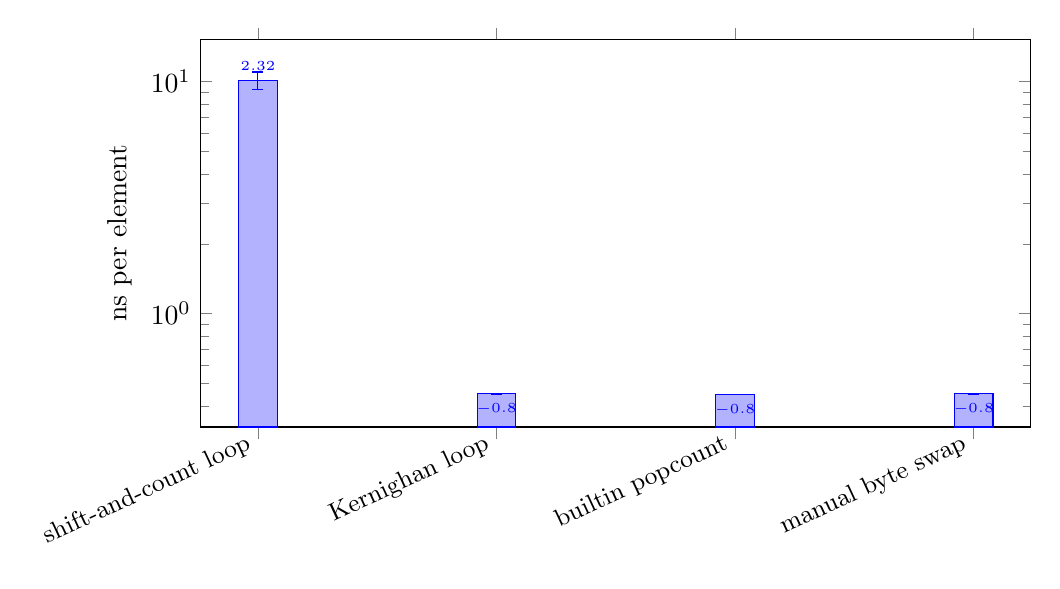
\begin{tikzpicture}
\begin{axis}[ybar, width=\textwidth, height=6.5cm, bar width=14pt, ymode=log, log origin=infty, symbolic x coords={shift-and-count loop,Kernighan loop,builtin popcount,manual byte swap}, xtick=data, x tick label style={rotate=25, anchor=east, font=\small}, ylabel={ns per element}, enlarge x limits=0.08, legend style={font=\small, at={(0.98,0.98)}, anchor=north east}, nodes near coords, nodes near coords style={font=\tiny}, every node near coord/.append style={/pgf/number format/.cd, fixed, precision=2}]
\addplot+[error bars/.cd, y dir=both, y explicit] coordinates {(shift-and-count loop,10.1445) +- (0,0.8638) (Kernighan loop,0.4507) +- (0,0.0013) (builtin popcount,0.4483) +- (0,0.0013) (manual byte swap,0.4507) +- (0,0.0013)};
\end{axis}
\end{tikzpicture}